\subsection{Hardware - V1.1}

    The switch module allows to switch 230V devices on and off and measure the current draw. 
    This module can not be compined with any other module. The switch module has two revisions,
    V1.0 and V1.1.

    Following components are required to fulfill the requirements:

    \begin{itemize}
        \item 1. Power-Supply
        \item 2. Switch
        \item 3. Current-Sensor
     
    \end{itemize}

    \subsubsection{Power-Supply}

        Because the switch module is switching 230V, it will also supplay itself with this voltage.
        A tranformer was chosen over a switching power supply because of the lower cost and the
        lower complexity.

        The used Transformer is from PLACEHOLDER with the type FL4/9 it has two 115V primary windings and
        two 9V secondary windings. The primary windings are connected in serial to the 230V mains and the
        secondary windings are connected in serial to a full-bridge rectifier. 

        \begin{figure}[H]
            \centering
            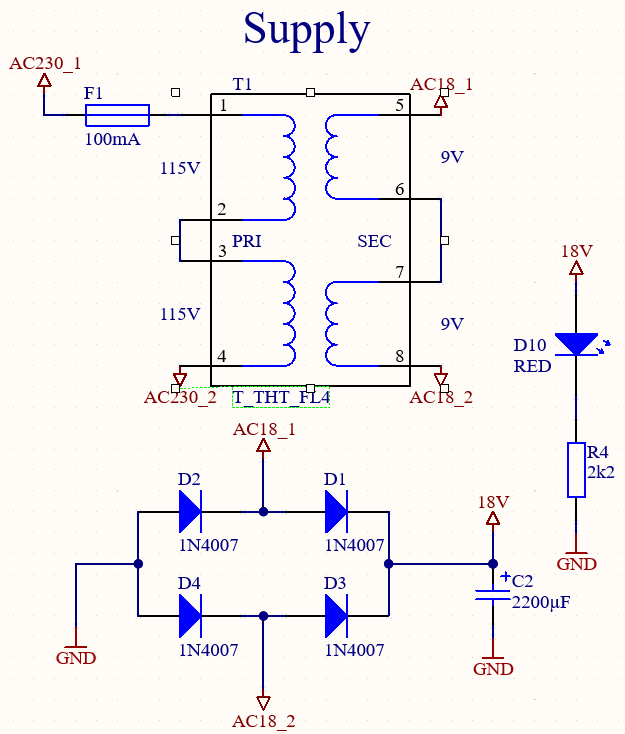
\includegraphics[width=0.5\textwidth]{assets/HW/Power-Supply-schematic.png}
            \caption{Power-Supply implemented in the schematic.}
        \end{figure}
        
        The output capacitor is calculated with the following formula:

        \begin{itemize}
            \item I ... Current draw
            \item $\Delta T$ ... Half the period of the frequency
            \item $\Delta U$ ... Ripple voltage
        \end{itemize}

        \begin{equation}
            C = \frac{I \cdot \Delta T}{\Delta U} = \frac{100mA \cdot 10ms}{0.5V} = 2mF
        \end{equation}

        The output voltage of 18V is stepped down to 12V with the LM2575 buck converter. The output
        voltage is set with a resistor divider to 12V. The 12V are needed to power the relay.

        The 12V are then stepped down to 5V with the LM7805 linear regulator. The base module and 
        current sensor are powered with the 5V.

         \begin{figure}[H]
            \centering
            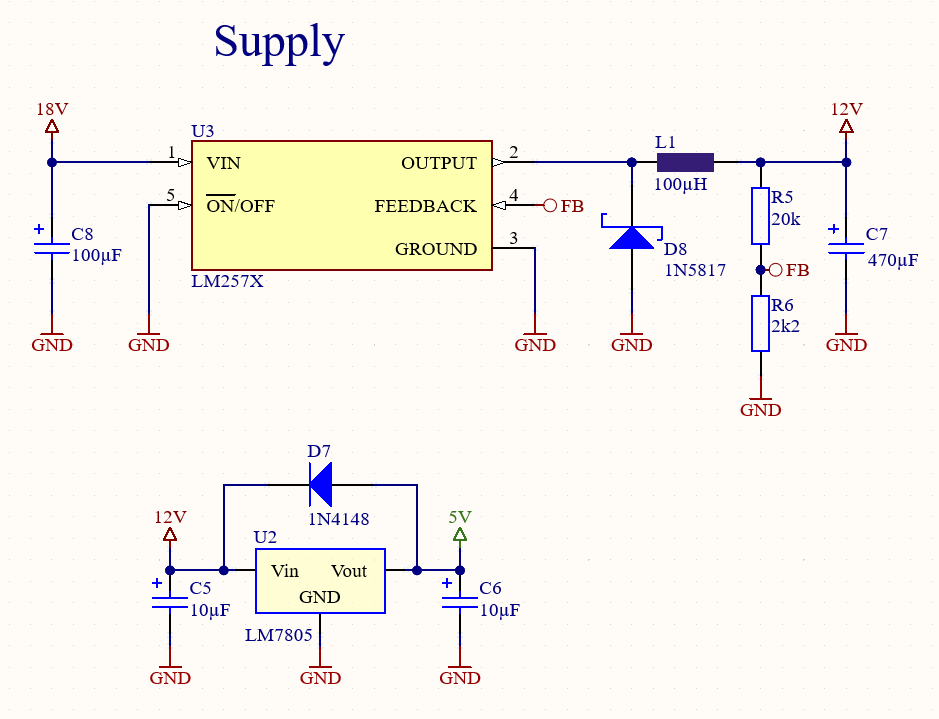
\includegraphics[width=0.8\textwidth]{assets/HW/Supply-schematic.png}
            \caption{Power-Supply implemented in the schematic.}
         \end{figure}

    \subsubsection{Relay}
        The switch module uses a relay to switch the 230V devices on and off. The relay used is 
        the JW1aFSN from Panasonic. The relay is controlled by a transistor and a flyback diode
        to protect the transistor from the voltage spike when the relay is switched off. The relay
        is rated for 10A at 250VAC. A LED was added to the relay to indicate the state of the relay. 
        The LED is connected to the port of the microcontroller and a resistor to limit the current.

        \begin{figure}[H]
            \centering
            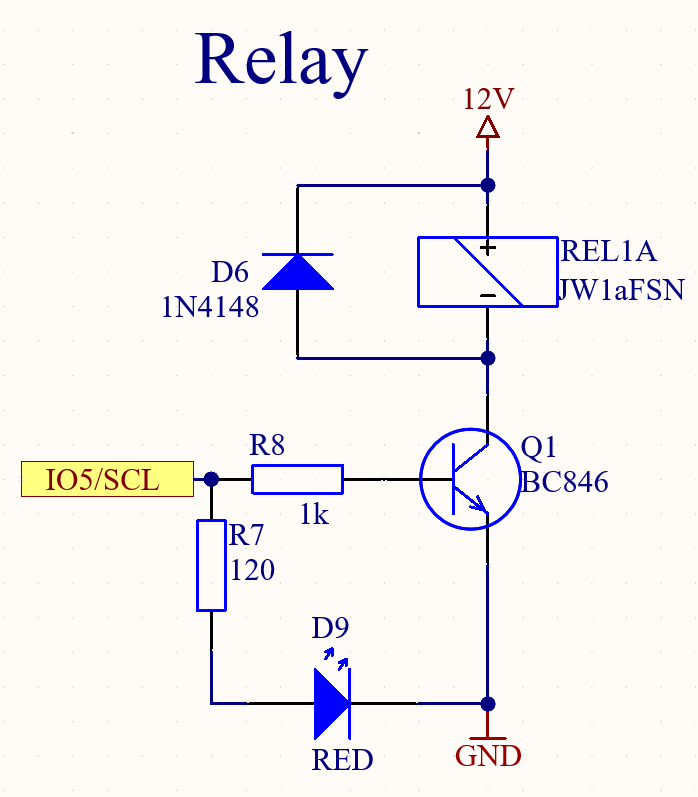
\includegraphics[width=0.4\textwidth]{assets/HW/Relay-Coil-schematic.png}
            \caption{Switch implemented in the schematic.}
        \end{figure}

        The relay is normally open. A connection is made from J1 to J2, when the coil is energized.

        \begin{figure}[H]
            \centering
            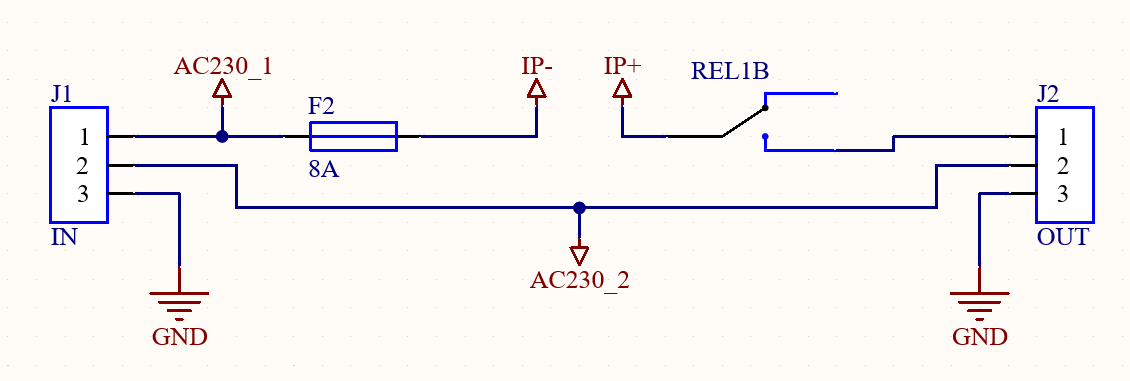
\includegraphics[width=0.8\textwidth]{assets/HW/Relay-Contact-schematic.png}
            \caption{Switch implemented in the schematic.}
        \end{figure}
    
    \subsubsection{Current-Sensor}

        The current sensor is used to measure the current draw of the switched device. The current
        sensor used is the ACS712ELCTR-20A-S from Allegro. The sensor is rated for 20A and has a 
        sensitivity of 100mV/A. The sensor is connected to the microcontroller over an analog pin.

        The available versions of the sensor were capably of measuring +-5A, +-20A and +-30A. 
        The 20A version was chosen because it covers the current range of the relay. 

        \begin{figure}[H]
            \centering
            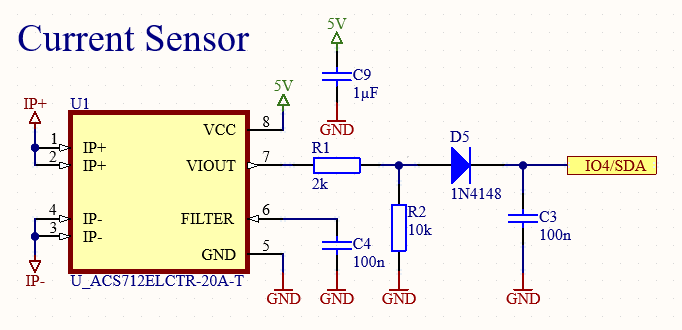
\includegraphics[width=0.8\textwidth]{assets/HW/Current-Sensor-schematic.png}
            \caption{Current-Sensor implemented in the schematic as shown in the datasheet \cite{noauthor_acs712_2024}.}
        \end{figure}

        The sensor is embedded in the current path of the relay. The terminals are 
        electrically isolated from the signal pins like described in the datasheet \cite{noauthor_acs712_2024}. 

        The IC is powered with 5V and the output on VIOUT is 2.5V when no current and 4.5V when 
        20A is flowing. In Order to adapt the output to the 3.3V ADC of the ESP32, a voltage divider
        is used like shown in the datasheet. The output is then connected to the ADC of the ESP32.

        \subsubsection{PCB}

        During the design of the PCB the espact of the 230V was considered. The PCB is divided
        into to sections, the 230V section and the <18V section. In the 230V section the relay, 
        current sensor ans the tranformer are placed. 
        Underneath the current sensor is a milled slot to ensure the isolation of the terminals. 
        
        \begin{figure}[H]
            \centering
            
\includegraphics[width=0.8\textwidth]{assets/HW/TBD.png}
            \caption{Cutout to prevent leakage current.}
        \end{figure}

        The PCB has a size of 100x92+mm. The switch module uses both SMD and THT components. It was decided to use more THT 
        components on this module, because most parts were allready available as THT.

        \begin{figure}[H]
            \centering
            
\includegraphics[width=0.8\textwidth]{assets/HW/TBD.png}
            \caption{PCB of the switch module V1.1 [Blue - Backside, Red - Frontside].}
        \end{figure}


\subsection{Hardware - V1.0}

    This version of the switch module is almost identical to the V1.1. Only minor changes were made
    to ensure the functionality of the module:

    \subsubsection{Relay}
    The base resistor of the transistor was forgotten in the schematic. The transistor was destroyed
    when the MCU pulled the port high. To prevent this in V1.1, a base resistor was added to limit 
    the current.

    \subsubsection{Power-Supply}
    While testing the module it was found that it is nowhere shown when 230V is present. Therefore
    a LED was added after the rectifier to indicate the presence of 230V.

    \subsubsection{Footprint}
    Footprints were changed in size to ensure the correct fit of the components.

    \subsubsection{PCB}
       

        \begin{figure}[H]
            \centering
            
\includegraphics[width=0.8\textwidth]{assets/HW/TBD.png}
            \caption{PCB of the switch module V1.1 [Blue - Backside, Red - Frontside].}
        \end{figure}